\documentclass[12pt,a4paper]{article}
\usepackage{amsmath,amssymb}
\usepackage{booktabs}
\usepackage{geometry}
\usepackage{graphicx}
\usepackage{float}
\usepackage{listings}
\usepackage{xcolor}
\usepackage{algorithm}
\usepackage{algpseudocode}
\usepackage{titlesec}
\usepackage{setspace}
\usepackage{ragged2e}

%----------------------------------------
% Page Setup for A4
%----------------------------------------
\geometry{
  a4paper,
  top=1in,
  bottom=1in,
  left=1in,
  right=1in
}

\setstretch{1.2}

%----------------------------------------
% Section title formatting
%----------------------------------------
\titleformat{\section}
  {\normalfont\bfseries\fontsize{14}{14}\selectfont}
  {\thesection}{1em}{}

%----------------------------------------
% Code listing style
%----------------------------------------
\lstdefinestyle{matlabstyle}{
  language=Matlab,
  basicstyle=\ttfamily\footnotesize,
  keywordstyle=\color{blue}\bfseries,
  commentstyle=\color{green!60!black},
  stringstyle=\color{orange!80!black},
  frame=none,
  numbers=none,
  breaklines=true,
  showstringspaces=false,
  tabsize=2
}

%----------------------------------------
\begin{document}

%----------------------------------------
% Cover Page
%----------------------------------------
\begin{titlepage}
\centering

\vspace*{0.5cm}
\includegraphics[width=0.22\textwidth]{diu_logo.png}\par
\vspace{0.5cm}

{\Large \textbf{Department of Computer Science and Engineering} \par}
\vspace{0.2cm}
{\Large \textbf{Dhaka International University} \par}

\vspace{0.8cm}

{\normalsize
Semester: 12th \par
Lab Report No: 01 \par
Course Code: CSE-420 \par
Course Title: Image Processing Lab \par
Report Title: Basic Image Processing Operations in MATLAB \par
}

\vspace{1cm}

{\Large \textbf{Submitted By} \par}
\vspace{0.3cm}

{\normalsize
Rasheduzzaman Rakib \par
Reg. No.: CS-D-77-22-120080 \par
Roll: 37 \par
Batch: D-77 \par
Department of Computer Science and Engineering \par
Dhaka International University \par
}

\vspace{1cm}

{\Large \textbf{Submitted To} \par}
\vspace{0.3cm}

{\normalsize
Md. Muksit Ul Islam \par
Assistant Professor \par
Department of Computer Science and Engineering \par
Dhaka International University \par
}

\vfill

{\normalsize Submission Date: 25th September 2026 \par}
{\normalsize Summer 2026 \par}

\end{titlepage}


%----------------------------------------
% Lab Report
%----------------------------------------

\section{Name}

\textbf{Basic Image Processing Operations in MATLAB}\\[0.3em]
Topics covered: Image Reading, RGB to Grayscale Conversion, Binary Conversion,
Image Resizing, Histogram Plotting, Crop/ROI, Image Rotation,
Brightness Enhancement, and Negative Image.

%----------------------------------------

\section{Description}

This lab introduces fundamental image processing operations using MATLAB's
Image Processing Toolbox. The built-in image \texttt{peppers.png} is used as
the input throughout all operations. The nine operations performed are briefly
described below.

\begin{enumerate}
  \item \textbf{Image Reading:} The original RGB colour image is loaded from
        disk using \texttt{imread} and displayed using \texttt{imshow}.

  \item \textbf{RGB to Grayscale:} \texttt{rgb2gray} converts the three-channel
        RGB image into a single-channel intensity image by computing a
        luminance-weighted average of the R, G, and B channels.

  \item \textbf{Binary Conversion:} \texttt{im2bw} thresholds the image at the
        default level of $0.5$ (on the $[0,1]$ normalised scale), producing a
        two-tone black-and-white image.

  \item \textbf{Resize:} \texttt{imresize} scales the image to a fixed
        $300\times300$ pixel resolution using bicubic interpolation.

  \item \textbf{Histogram:} \texttt{imhist} computes and plots the pixel
        intensity frequency distribution of the grayscale image, giving insight
        into contrast and tonal range.

  \item \textbf{Crop / Region of Interest (ROI):} \texttt{imcrop} extracts a
        $200\times160$ pixel rectangular patch starting at pixel $(50,50)$,
        isolating a specific region of interest.

  \item \textbf{Rotation:} \texttt{imrotate} rotates the image by $45^\circ$
        counter-clockwise. Pixels that fall outside the original frame are
        filled with black (zero-padding).

  \item \textbf{Brightness Enhancement:} A scalar value of $100$ is added to
        every pixel using \texttt{I + 100}. MATLAB's saturation arithmetic
        clamps values that exceed $255$, brightening the overall image.

  \item \textbf{Negative Image:} The complementary image is computed as
        $255 - I$, inverting each pixel's intensity and producing a
        photographic negative effect.
\end{enumerate}

%----------------------------------------

\section{Code}

\begin{lstlisting}[style=matlabstyle]
% 1. image reading
I = imread('peppers.png');
figure;
subplot(3,3,1);
imshow(I);
title('original image');

% 2. rgb to grayscale
gr = rgb2gray(I);
subplot(3,3,2);
imshow(gr);
title('grayscale');

% 3. binary conversion
BW = im2bw(I);
subplot(3,3,3);
imshow(BW);
title('binary image');

% 4. resize
rsz = imresize(I, [300 300]);
subplot(3,3,4);
imshow(rsz);
title('resized image');

% 5. histogram
subplot(3,3,5);
imhist(gr);
title('histogram');

% 6. crop or roi
crop = imcrop(I, [50 50 200 160]);
subplot(3,3,6);
imshow(crop);
title('crop or roi');

% 7. rotation
rot = imrotate(I, 45);
subplot(3,3,7);
imshow(rot);
title('rotated image');

% 8. brightness enhancement
bright = I + 100;
subplot(3,3,8);
imshow(bright);
title('brightness +100');

% 9. negative image
negative = 255 - I;
subplot(3,3,9);
imshow(negative);
title('negative image');
\end{lstlisting}

%----------------------------------------

\section{Output}

The figure below presents all nine processed outputs arranged in a $3\times3$
subplot grid, as produced by running \texttt{lab\_01.m} in MATLAB.

\begin{figure}[H]
  \centering
  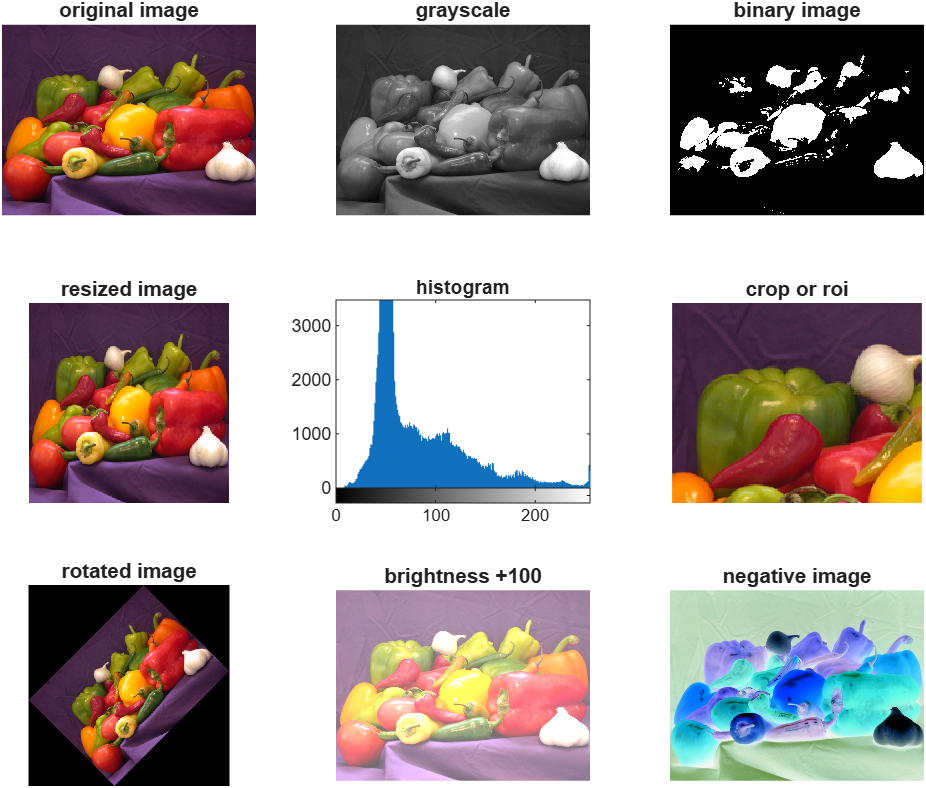
\includegraphics[width=0.82\textwidth]{Figure_1.png}
  \caption{Nine image processing operations on \texttt{peppers.png}}
  \label{fig:output}
\end{figure}

Figure~\ref{fig:output} confirms all nine operations executed correctly:
colour space conversions (subplots 2--3), spatial transforms (4, 6, 7),
intensity analysis (5), and pixel-level arithmetic (8--9) all produce
the expected results on the \texttt{peppers.png} test image.

\end{document}
